\Cref{sec:fitting_mbc,sec:background_subtraction} introduced the fitting procedure and \BB background subtraction.
Together with the optimal selections from \Cref{sec:final_optimisation}, this fully defines the analysis strategy from the Belle~II simulated datasets to the \BtoXsgamma spectrum.
However, the defined fitter has to be validated in simulation to give an unbiased estimation of \BtoXsgamma events, with a good resoltion and signal efficiency.
The studies in this Section will show such results.

\subsection{Validation of \texorpdfstring{\Mbc}{Mbc} fit on reduced samble size}\label{sec:mbc_fit_validation_misreconstructed}

The results that were shown in \Cref{fig:mc_fit_yield_comparisons} only provided results for fitting 1.6~\invab -- a dataset about an order of magnitude larger than is expected in the case of this analysis.
Therefore, the generic \MC dataset is pseudorandomly split into 10 smaller subsets, corresponding to 160~\invfb, and each of them are fitted independently.
The choice of 160~\invfb, rather than 190~\invfb which is the sample size of the Belle~II data used in the analysis, is due to anticipated data-simulation differences.
\todo[inline]{see XXX and next paragraph performed where?}
Indeed, a 190~\invfb dataset should correspond to roughly 160~\invfb in simulation due to differences in tag-\B reconstruction efficiency.

The resulting 10 fits and the estimated $\mathcal{N}_{CB}$ corresponding to each \EB bin are shown in \Cref{fig:extracted_validation_mc}.
The expected number of events in each fit is always equal to one tenth of that in the total generic \MC dataset.
It can be observed that all data points, and their average, are statistically compatible with the expectation.
These results indicate, that despite using a 10 times larger dataset to define the \PDF{s}, this \Mbc fit model produces reliable results.
Further tests, particularly a test ensuring that the fitter is unbiased, are performed later.

\begin{figure}[htbp!]
    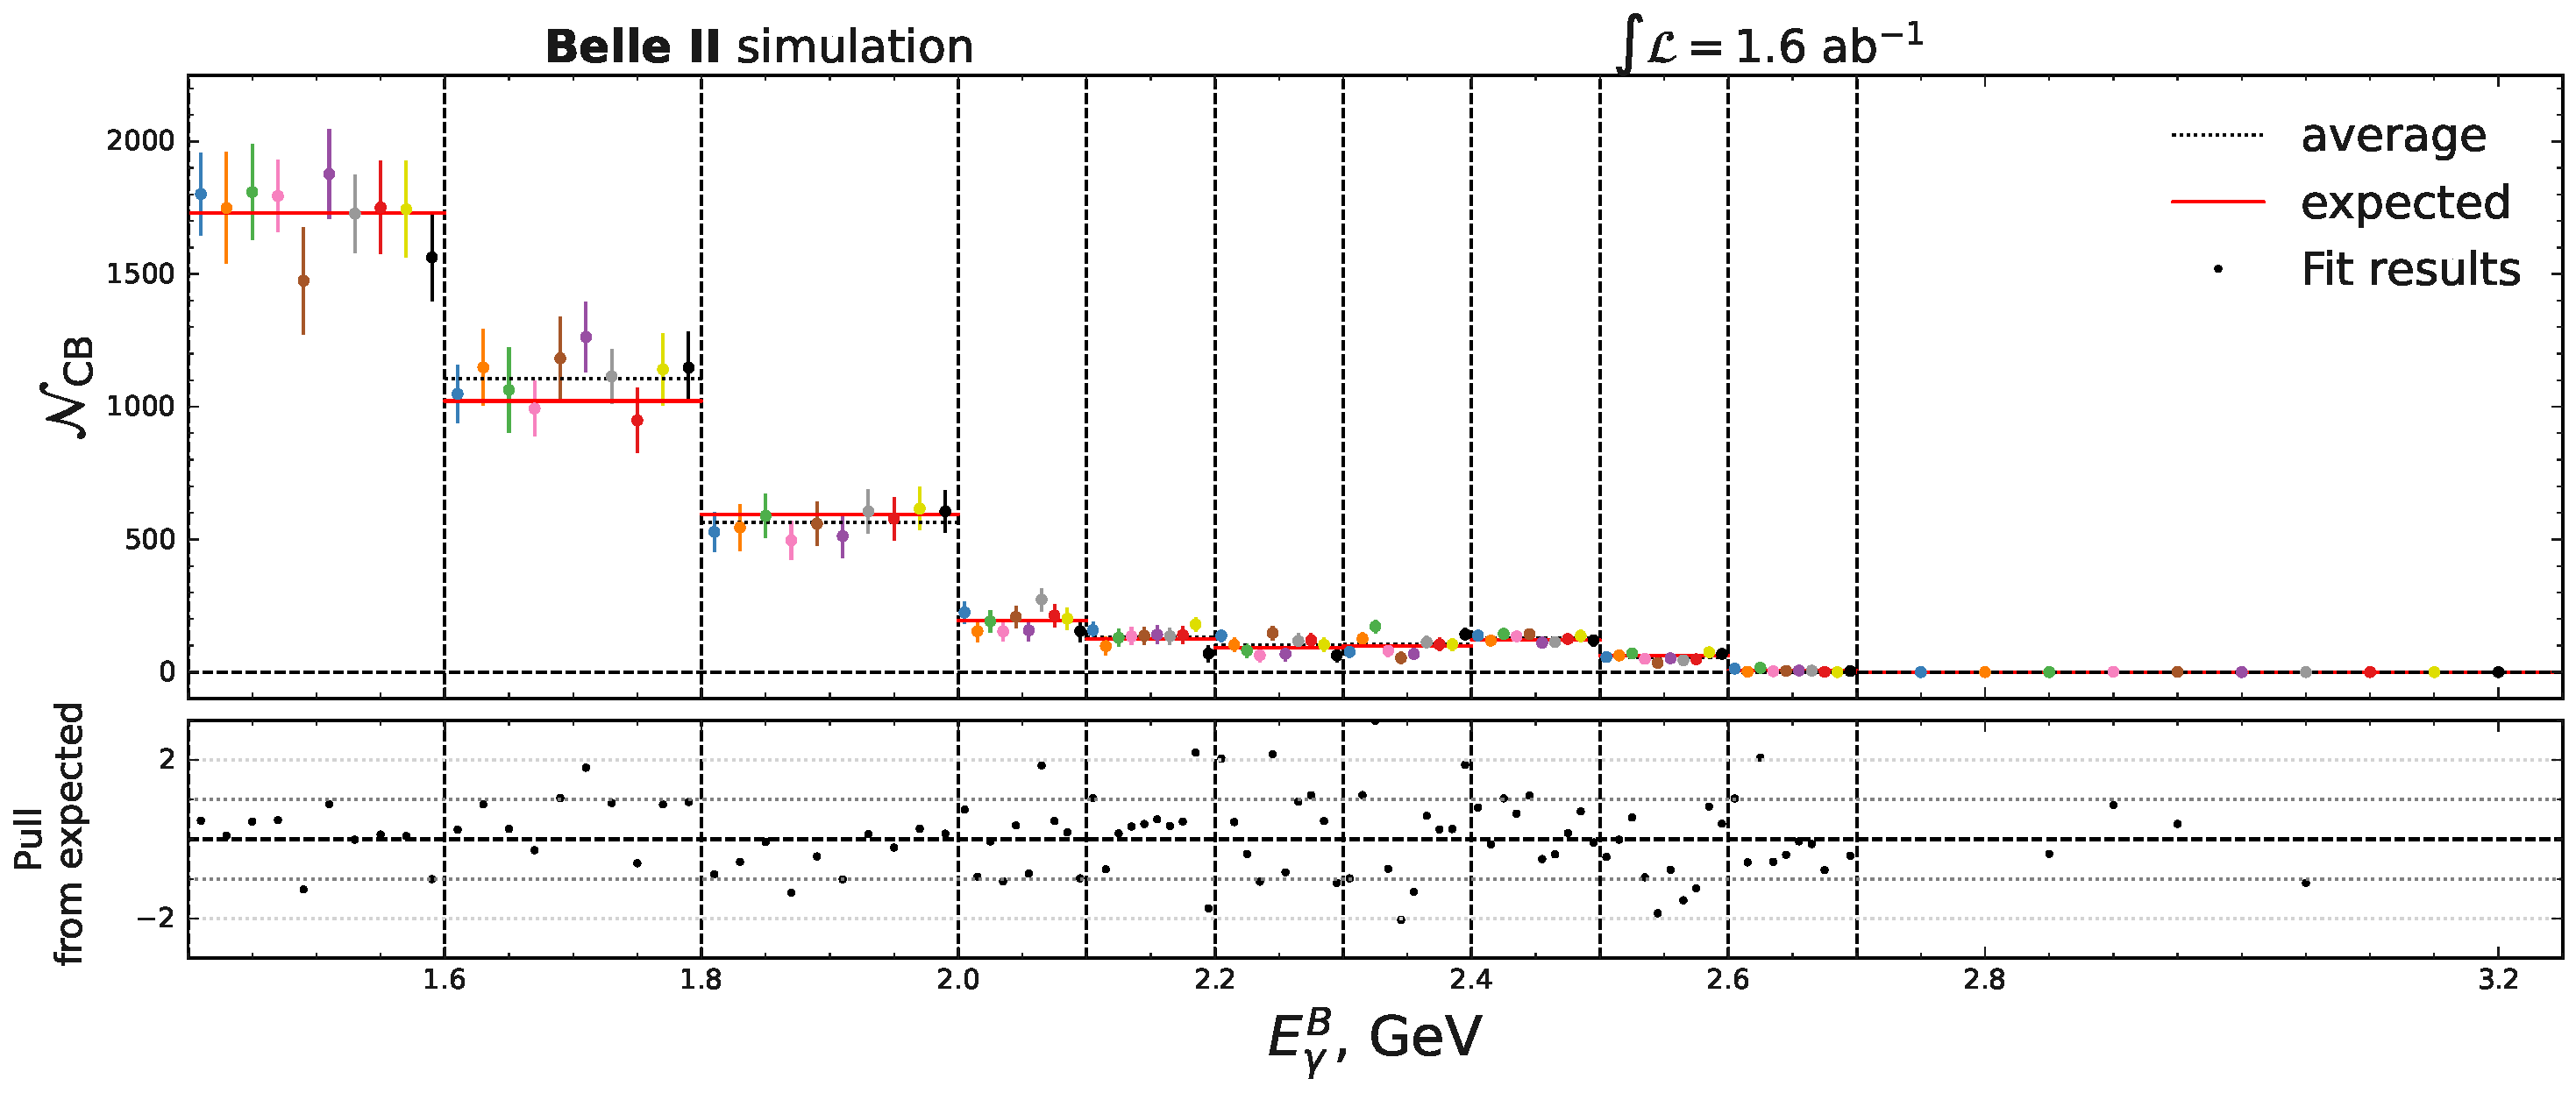
\includegraphics[width=0.9\textwidth]{figures/mc_validation/extracted_signal_generic_mc.pdf}
    \caption{\label{fig:extracted_validation_mc}The estimated $\mathcal{N}_{CB}$ values from fits on one tenth of generic \MC, corresponding to 160~\invfb of simulation.
    The dashed lines represent different \EB bins, each bin showing one data point corresponding to a simultaneous fit of all \EB bins.
    The dotted lines show the average of all 10 points in each bin, whereas the full lines show the number of good tag-\B events in the original 1.6~\invab dataset, scaled down 10 times (`expected').
    The subpanels show the pull of each datapoint from the expected number of events.
    These results show that the fit is able to extract a result on a dataset that is an order of magnitude smaller.
    }
\end{figure}

\subsection{Validation of subtraction of remaining-\texorpdfstring{\BB}{BB} background}\label{sec:background_subtraction_validation_mc}

The strategy to extract the \BtoXsgamma photon energy spectrum and suppress the remaining \BB background was laid out in \Cref{sec:background_subtraction}.
In particular, full generic \MC dataset is modified, such that no-\BtoXsgamma events are present in it.
Then, the \Mbc fit discussed in \Cref{sec:fitting_setup} is performed.
To test that this procedure is viable, the subtraction is performed for the results shown in \Cref{fig:extracted_validation_mc}.
Although the 10 fits are performed on 160~\invfb datasets, the background subtraction is done with a 1.6~\invab dataset.
Therefore, the statistical uncertainty from the fit on the smaller dataset is dominating.
The subtracted result is shown in \Cref{fig:subtracted_validation_mc}.

\begin{figure}[htbp!]
    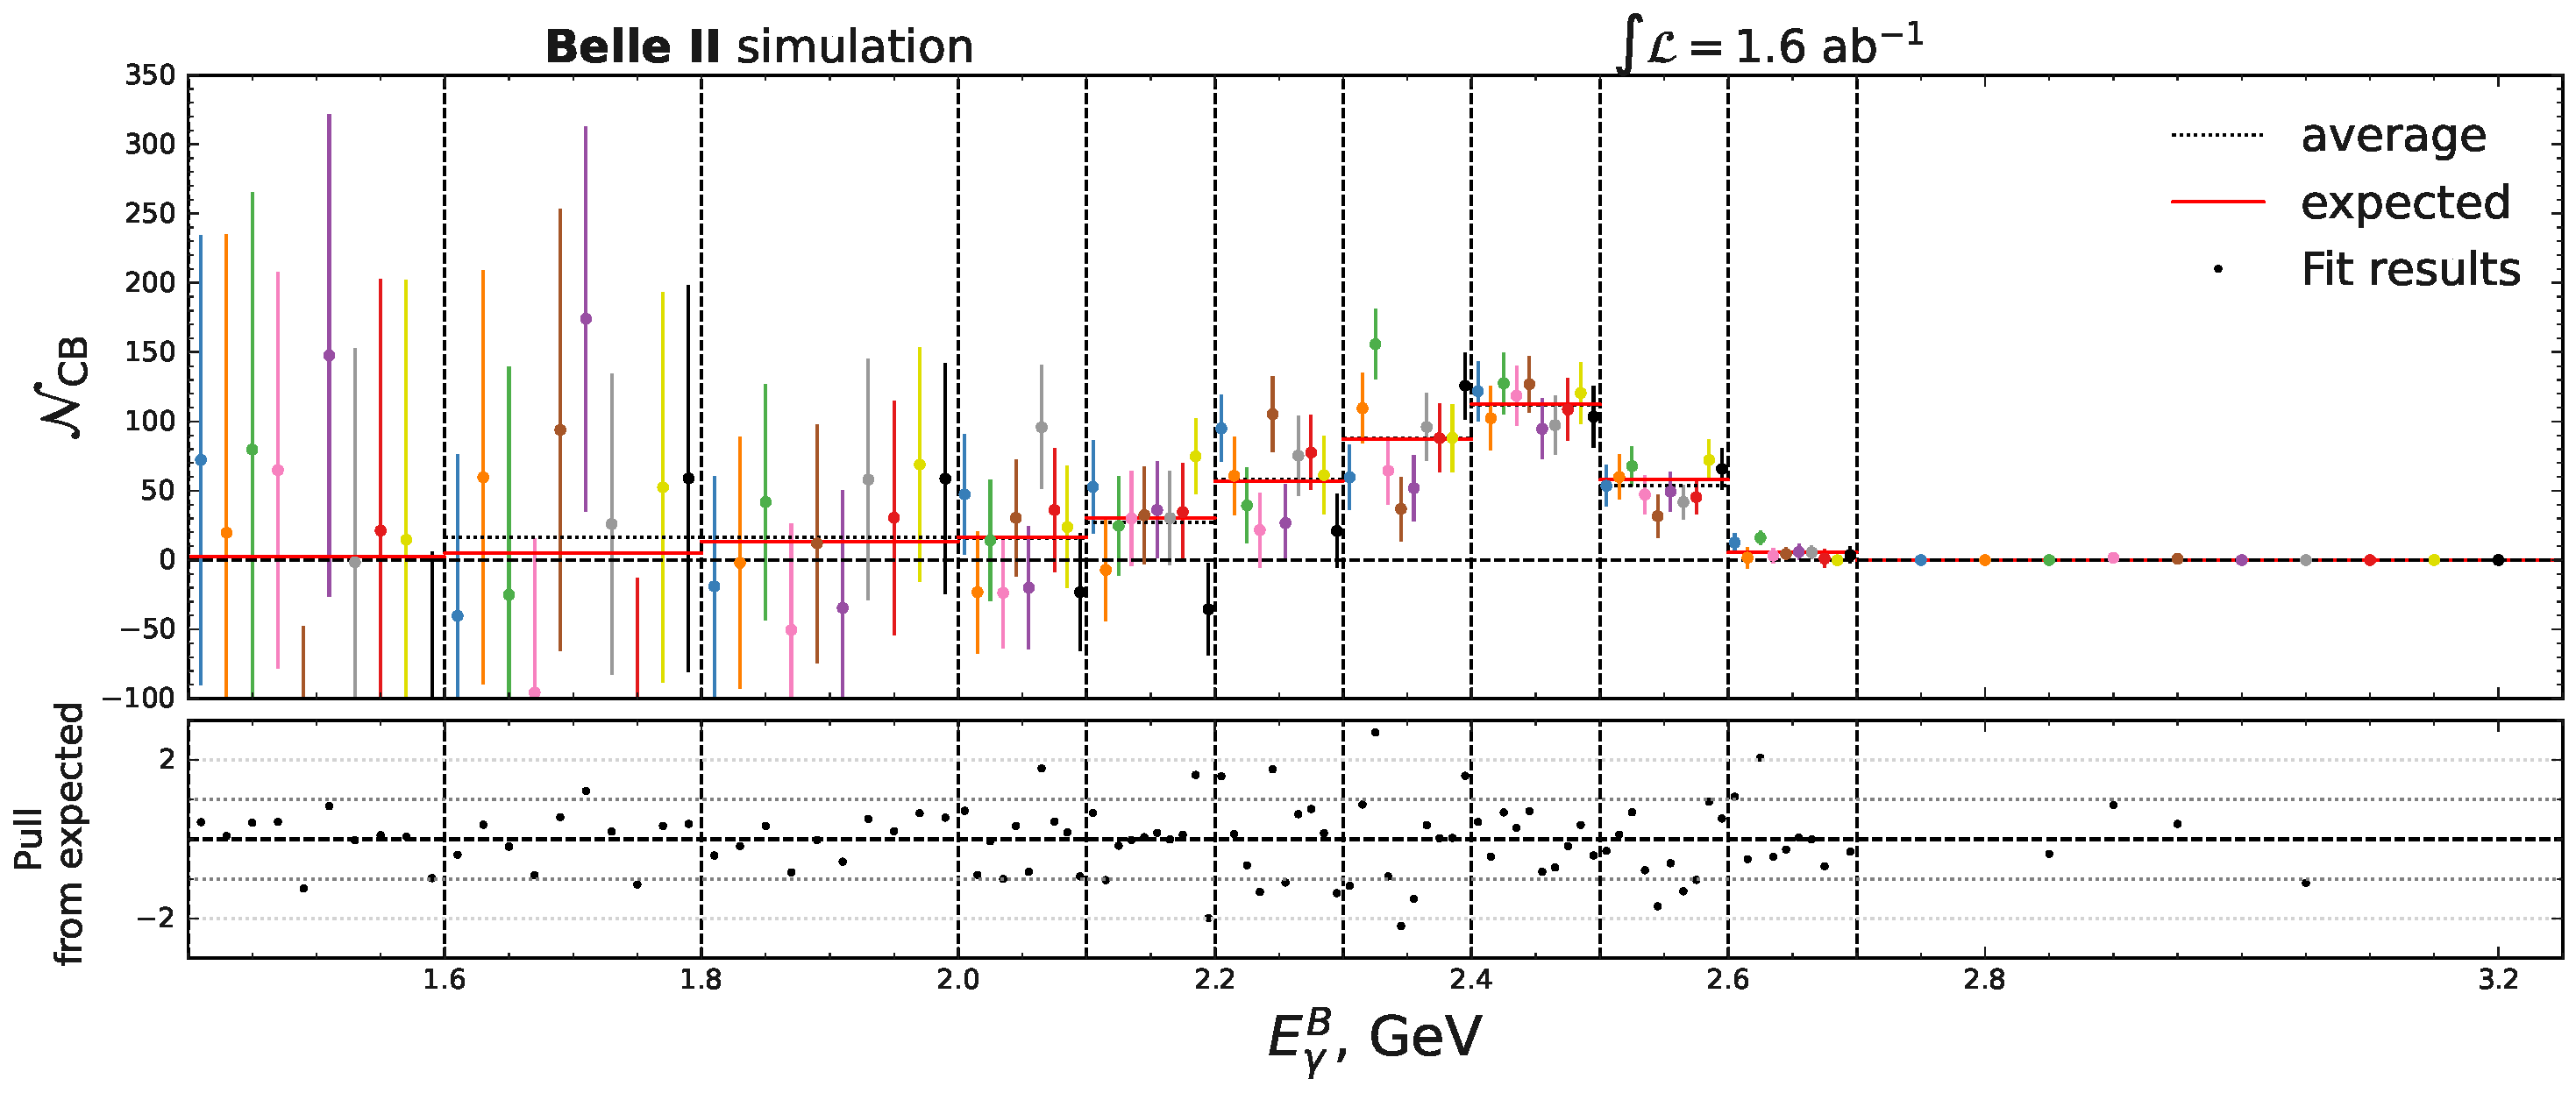
\includegraphics[width=0.9\textwidth]{figures/mc_validation/subtracted_signal_generic_mc.pdf}
    \caption{\label{fig:subtracted_validation_mc}
    The estimated $\mathcal{N}_{CB}$ with subtracted background, based on the \Cref{eq:background_subtraction}.
    The values before \BB-background subtraction are shown in a corresponding \Cref{fig:extracted_validation_mc}.
    To ensure that a minimal statistical background subtraction uncertainty is introduced, the full 1.6~\invab dataset is chosen to subtract the background.
    The uncertainties of each data point are those of the \Mbc fit on the background dataset and on the tested subset, added in quadrature.
    }
\end{figure}

The 1.6~\invab dataset and the 160~\invfb subsets are largely correlated, therefore the result has a smaller spread than one might expect from a unit Gaussian, based on the statistical ucnertainty provided by the fitter.
However, the purpose of this test is to showcase that the setup is able to extract values that are statistically compatible with the original dataset.
The results showcased in \Cref{fig:extracted_validation_mc,fig:subtracted_validation_mc} clearly show that the central values of the \EB spectrum extracted follow the number of \BtoXsgamma events in the dataset.
In this section so far, no particular modelling of \BtoXsgamma spectrm has been assumed.
In fact, following the tests from \Cref{fig:mc_fit_yield_comparisons}, it is clear that the analysis is \textit{so far} signal-model independent, as no direct assumptions have been made thus far.
On the other hand, following the setup that is taken to remove \BB backgrounds after the \Mbc fit, the analysis is heavily background-model dependent.
For this reason, special emphasis will be put on testing the \textit{background} description validation, as opposed to signal validation in later chapters XXXX.
\todo[inline]{later chapter xxxx}

\subsection{Closure test of the \texorpdfstring{\Mbc}{Mbc} fitter}\label{sec:closure_test}

If the uncertainties estimated by a fitter are correct, then fitting pseudodata sets generated from \PDF{s} fitted on test data must yield statistically compatible results.
This verifies two important aspects of the fitter:
\begin{itemize}
    \item the estimated parameter central values of the fitter are reproduced, when fitting a statistically equivalent dataset;
    \item the estimated parameter central values of the fitter are distributed accordingly to the uncertainties that the fitter provides.
\end{itemize}

More concisely, the pull distribution of an unbiased fitter, in this case calculated as:
\begin{equation}\label{eq:toy_pull}
    \mathrm{pull} = \frac{\mathcal{N}\times \mathrm{scale} - \mathcal{N}^{\mathrm{pseudo}}}{\mathrm{fit~error}},
\end{equation}
must be described by a unit Gaussian (assuming the central limit theorem is applicable for the psuedodata sample size).
In the case of this analysis, $\mathcal{N}_{\mathrm{CB}}$ is the estimated number of good tag-\B mesons in the generic-\MC sample.
The uncertainty, $\mathrm{fit~error}$ is a corresponding uncertainty, in this analysis estimated by the \texttt{HESSE} method.
On the other hand, $\mathcal{N}^{\mathrm{pseudo}}_{\mathrm{CB}}$ is a randomly sampled dataset that follows the \PDF{s} fitted on the generic-\MC dataset.
The $\mathrm{scale}$ is used to equate the sample size between the sampled and total simulated dataset.
Tests of this type are known as \textit{closure tests} is statistics and allow to verify that the central values reproduced by the fitter fluctuate as indicated by the \PDF uncertainties.

The closure test in this analysis is done on pseudodata sets of equivalent size as the Belle II collected data.
First, 1000 pseudodata sets equivalent to $\mathrm{160~\invfb}$ are sampled from the \PDF that was fitted in \Cref{fig:primary_full_fits}.
Since in all of the cases $\mathcal{N}_{\mathrm{CB}}$ and $\mathrm{fit~error}$ are known exactly, the \Mbc fitter is used on the pseudodata set, and a $\mathrm{pull}$ is calculated based on \Cref{eq:toy_pull}.
The pull distribution for every \EB bin are shown in XXX.
To test the statistical validity of \Mbc fits on each bin, a Gaussian \PDF is fitted on the distributions, with parameters $\mu$ and $\sigma$ being estimated.
The parameters correspond to the mean value, and the width of the Gaussian distribution, respectively.
The parameter estimation is performed as an unbinned negative log-likelihood fit.
The corresponding Gaussian fit result, and the parameters are also shown in XXX.
